\documentclass[showkeys,aps,prb,prepreint,amssymb, amsmath,nobibnotes]{article}
\usepackage{bm,setspace}
\usepackage{graphicx,graphics,booktabs}
\usepackage[a4paper,margin=2cm]{geometry}
\newlength{\dhatheight}
\begin{document}
\section{Raw data, ubiquitin, 500 MHz}

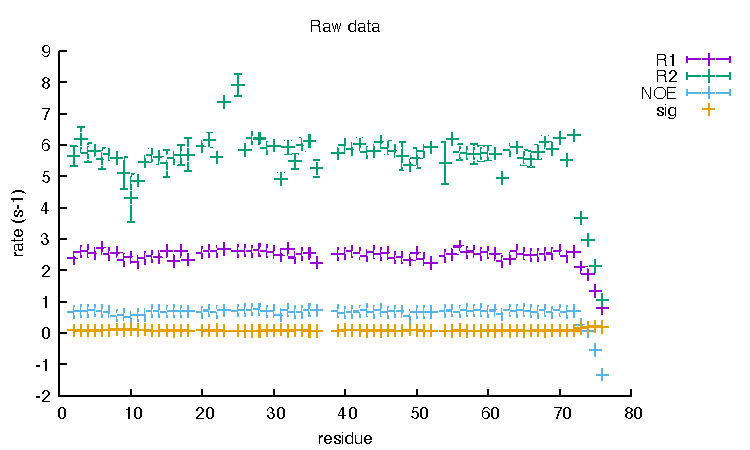
\includegraphics[width=0.495000\textwidth]{figraw}
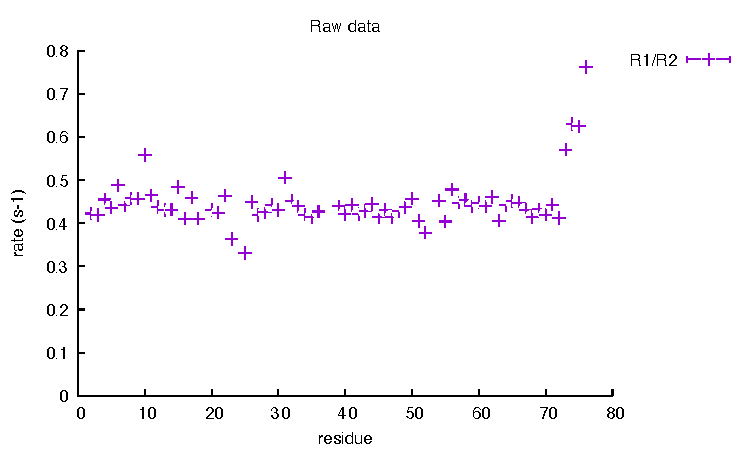
\includegraphics[width=0.495000\textwidth]{fig2raw}
\end{figure} 
\section{Computation of rates verus correlation time, Isotropic model}

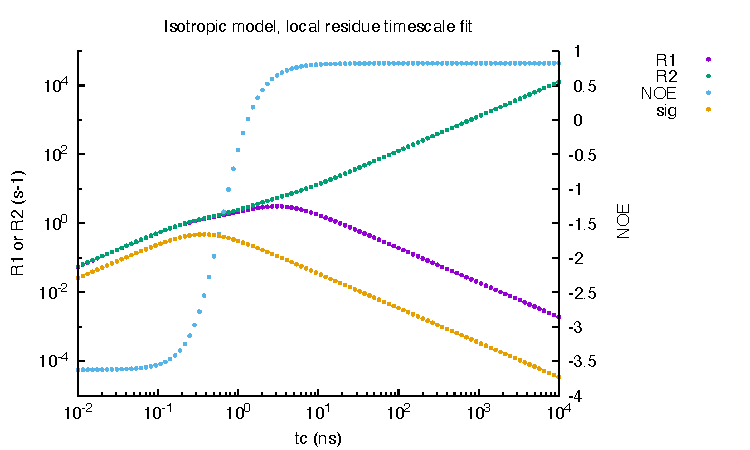
\includegraphics[width=0.495000\textwidth]{figCorr}
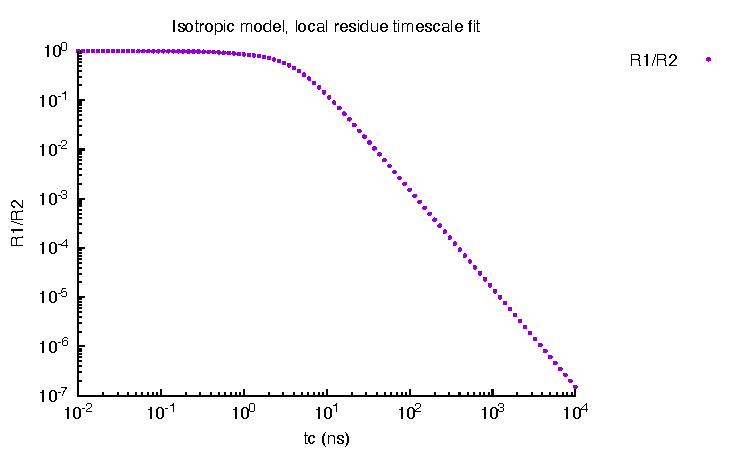
\includegraphics[width=0.495000\textwidth]{fig2Corr}
\end{figure} 
\section{Spectral density}

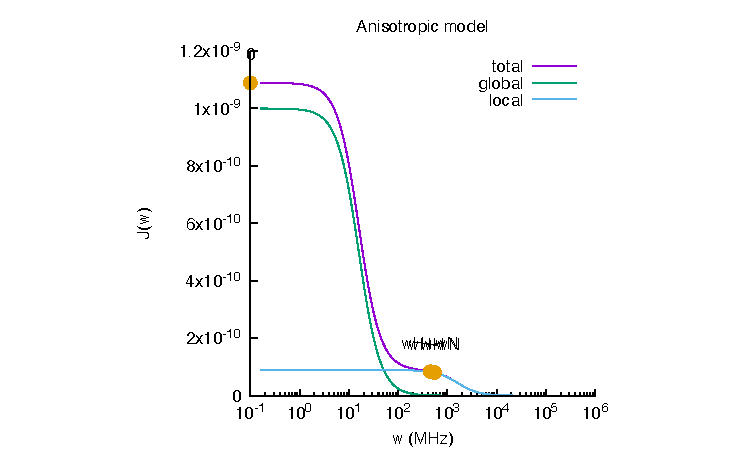
\includegraphics[width=0.495000\textwidth]{figJ1.pdf}
\end{figure} 
Simulated model free spectral density function with $S^2$ 0.10, global tumbling $10.00$ ns and local tumbling $0.10$ ns. The sampled frequencies are indicated by points and labelled.

\section{Isotropic model, local $\tau_c$ fit}

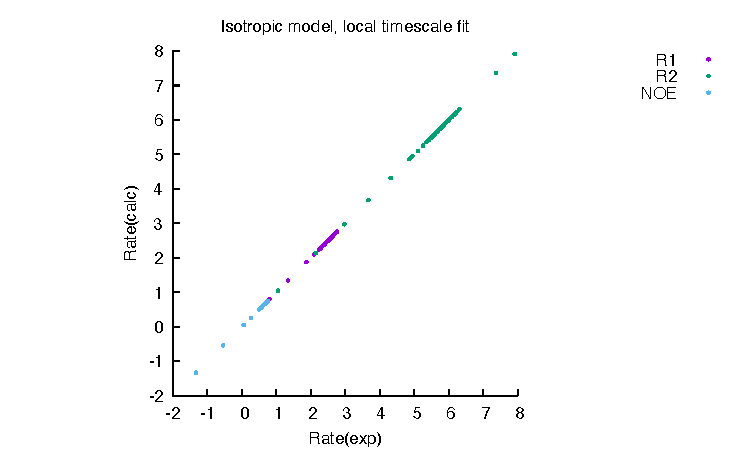
\includegraphics[width=0.330000\textwidth]{fig1.pdf}
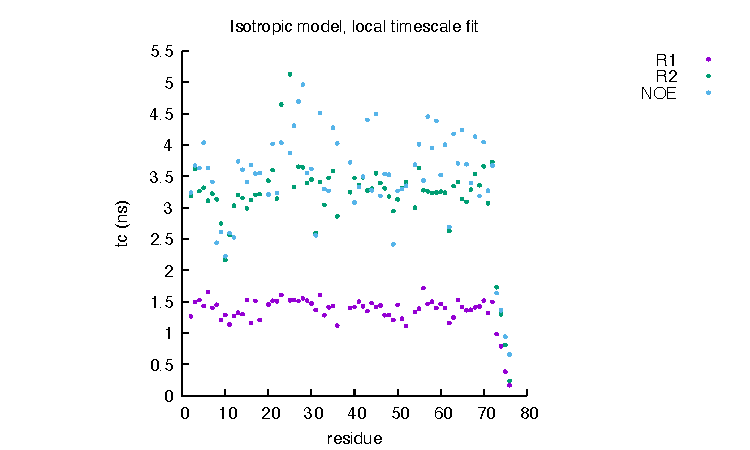
\includegraphics[width=0.330000\textwidth]{fig2.pdf}
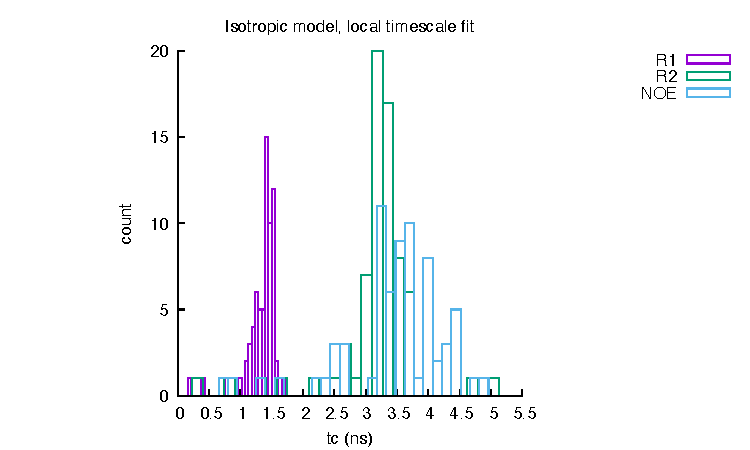
\includegraphics[width=0.330000\textwidth]{fig3.pdf}
\end{figure} 
\noindent Parameters $P$: 210

$\tau_c$ mean from R1 : 1.354 $\pm$ 0.242 ns

$\tau_c$ mean from R2 : 3.164 $\pm$ 0.669 ns

$\tau_c$ mean from NOE : 3.452 $\pm$ 0.801 ns

$\tau_c$ overall: 2.657 $\pm$ 1.116 ns

\noindent Datapoints $N$: 210

$\chi^2/N$: 0.000

$\chi^2/(N-P)$: inf

RMSD:   0.0000 s$^{-1}$

\section{Isotropic model, global $\tau_c$ fit}

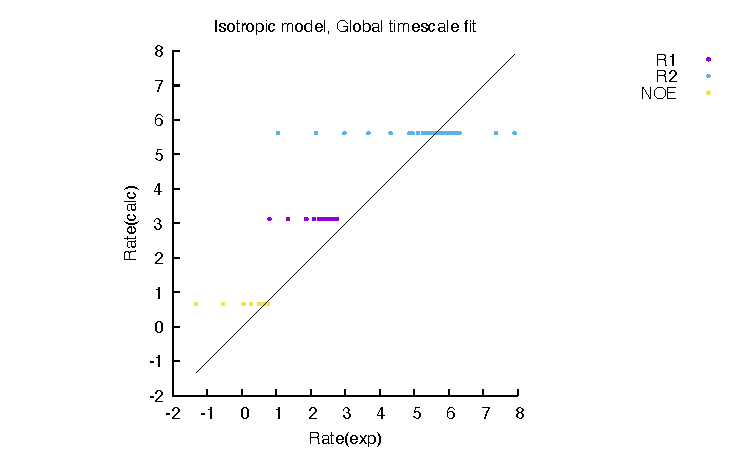
\includegraphics[width=0.495000\textwidth]{figGlob1.pdf}
\end{figure} 
\noindent Parameters $P$: 1

$\tau_c$ global: 3.151 ns

\noindent Datapoints $N$: 210

$\chi^2/N$: 430.602

$\chi^2/(N-P)$: 432.663

RMSD:   0.7039 s$^{-1}$

\section{Isotropic model, local residue $\tau_c$ fit}

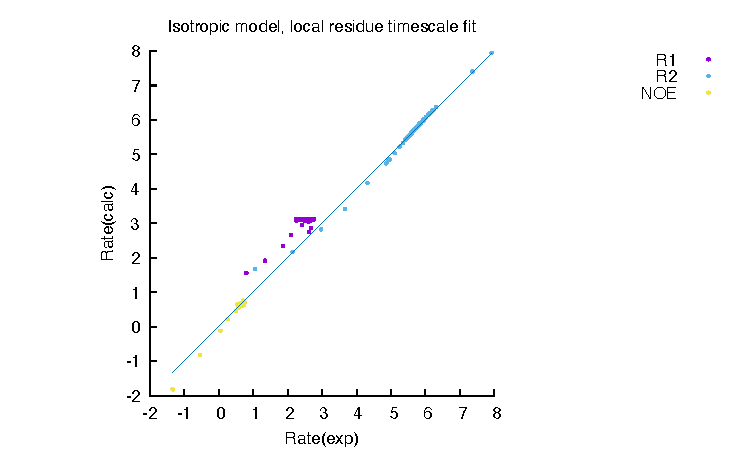
\includegraphics[width=0.330000\textwidth]{fig1res.pdf}
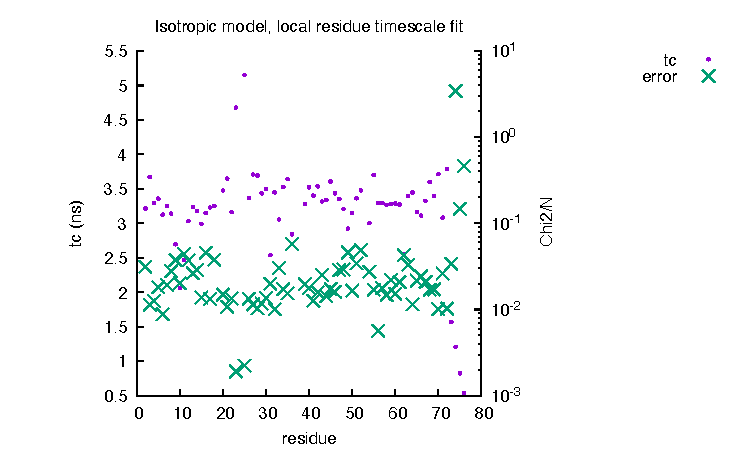
\includegraphics[width=0.330000\textwidth]{fig2res.pdf}
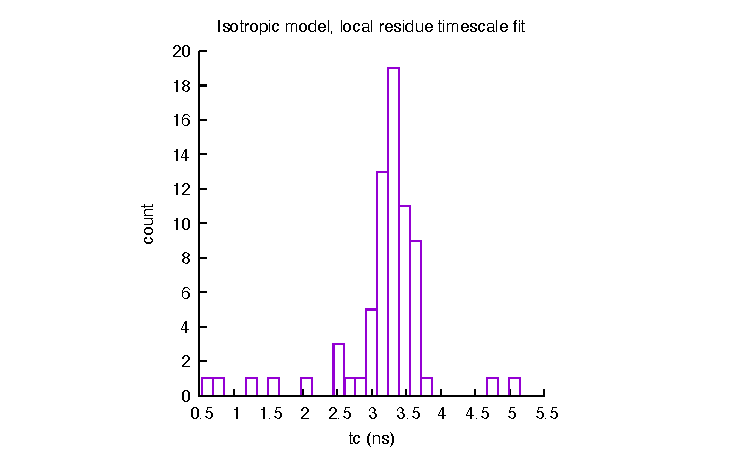
\includegraphics[width=0.330000\textwidth]{fig3res.pdf}
\end{figure} 
\noindent Parameters $P$: 70

$\tau_c$ residue overall: 3.190 $\pm$ 0.677 ns

\noindent Datapoints $N$: 210

$\chi^2/N$: 186.379

$\chi^2/(N-P)$: 279.569

RMSD:   0.3546 s$^{-1}$

\section{Model Free fit}

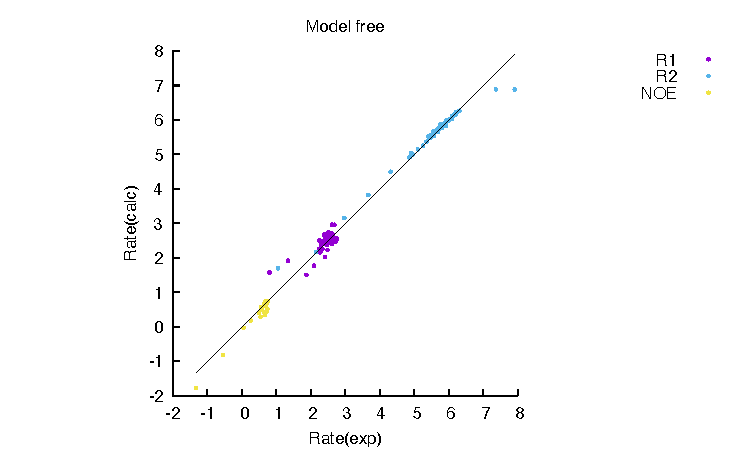
\includegraphics[width=0.495000\textwidth]{figGlobFree1.pdf}
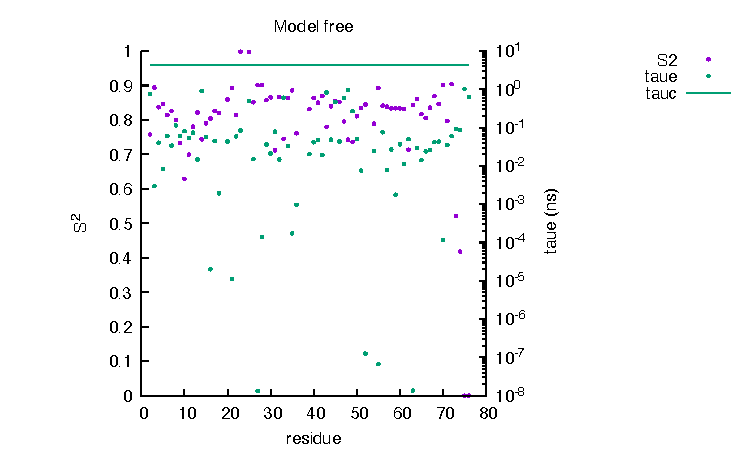
\includegraphics[width=0.495000\textwidth]{figGlobFree2.pdf}
\end{figure} 
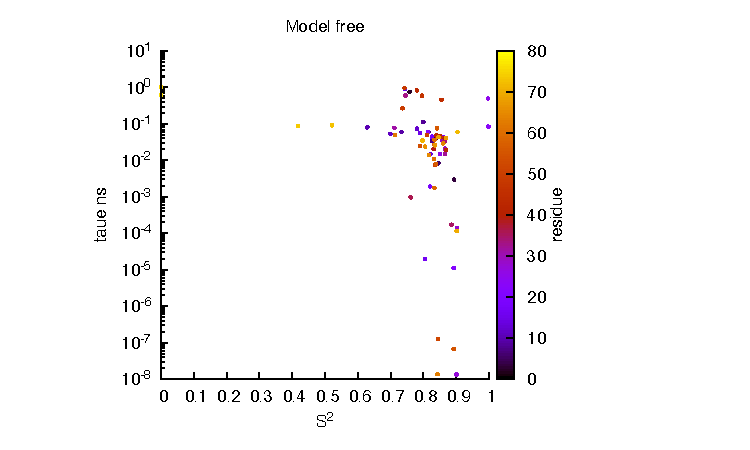
\includegraphics[width=0.495000\textwidth]{figGlobFree3.pdf}
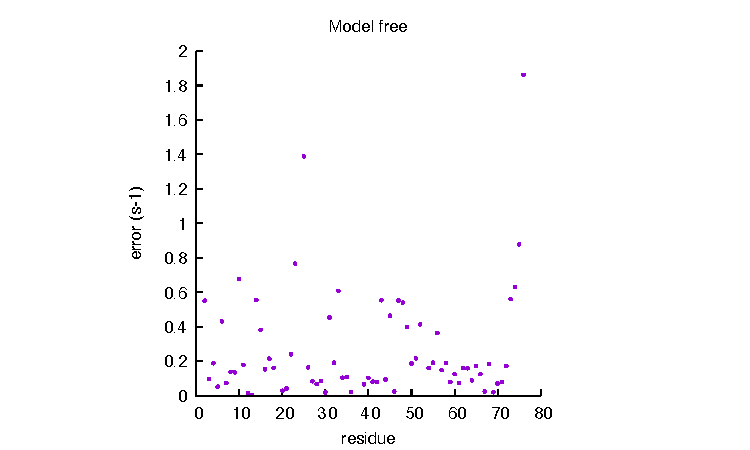
\includegraphics[width=0.495000\textwidth]{figGlobFree4.pdf}
\end{figure} 
\noindent Parameters $P$: 141

$\tau_c$ global: 4.236 ns

\noindent Datapoints $N$: 210

$\chi^2/N$: 31.582

$\chi^2/(N-P)$: 96.118

RMSD:   0.1600 s$^{-1}$

\section{Axial tumbling}

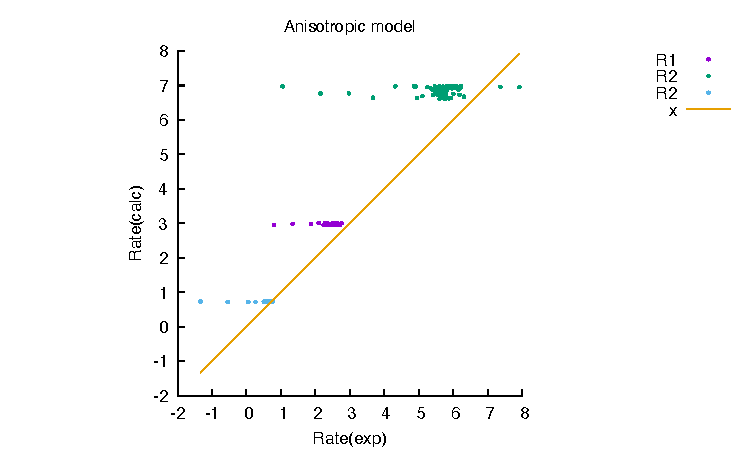
\includegraphics[width=0.330000\textwidth]{figanisoR1R2.1.pdf}
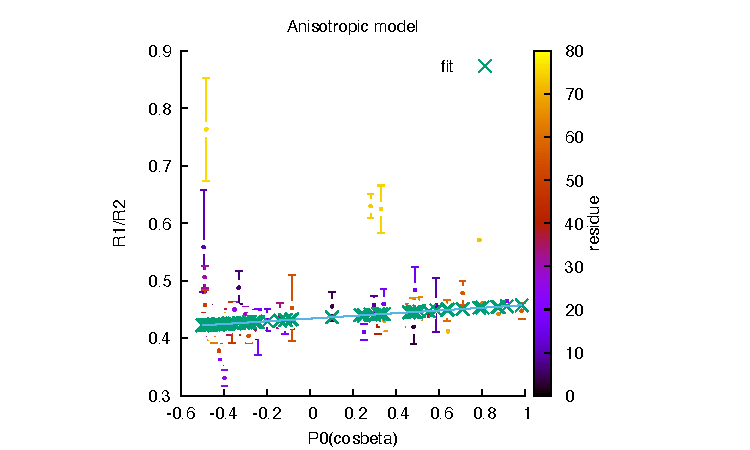
\includegraphics[width=0.330000\textwidth]{figanisoR1R2.2.pdf}
\end{figure} 
Fitting R1R2 ratio

\noindent Parameters $P$: 4

tshape: 1.18

tc:     3.97 ns

$M_\theta$: -1.25 degrees

$M_\phi$:     180.01 degrees

\noindent Datapoints $N$: 210

$\chi^2/N$: 435.272

$\chi^2/(N-P)$: 443.723

RMSD:   0.9809 s$^{-1}$

\section{Model Free Axial fit}

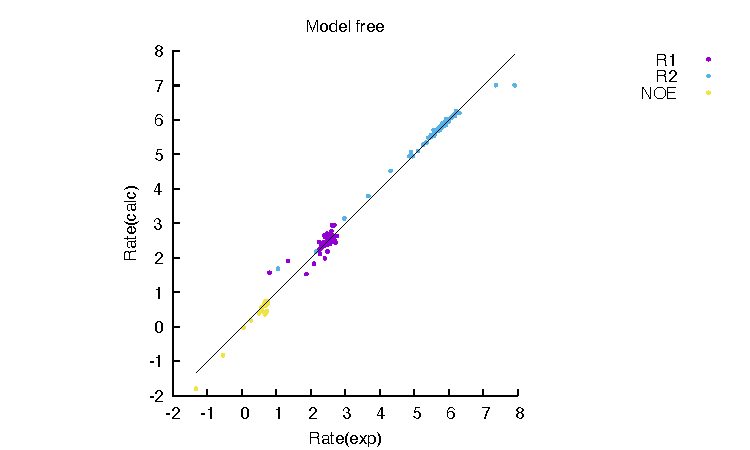
\includegraphics[width=0.495000\textwidth]{figGlobFreeAx1.pdf}
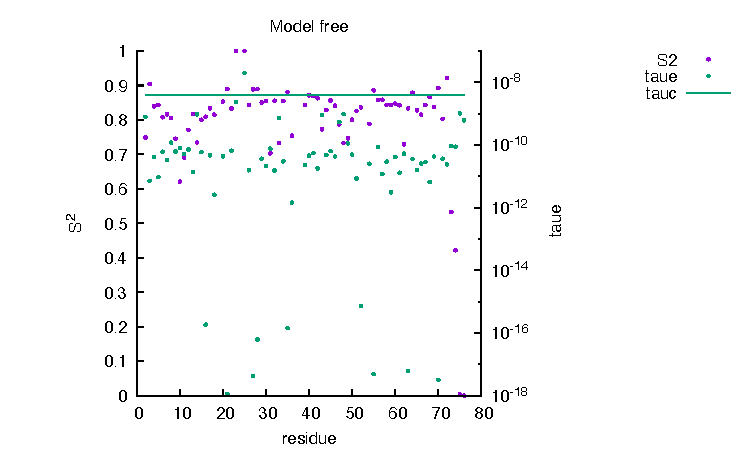
\includegraphics[width=0.495000\textwidth]{figGlobFreeAx2.pdf}
\end{figure} 
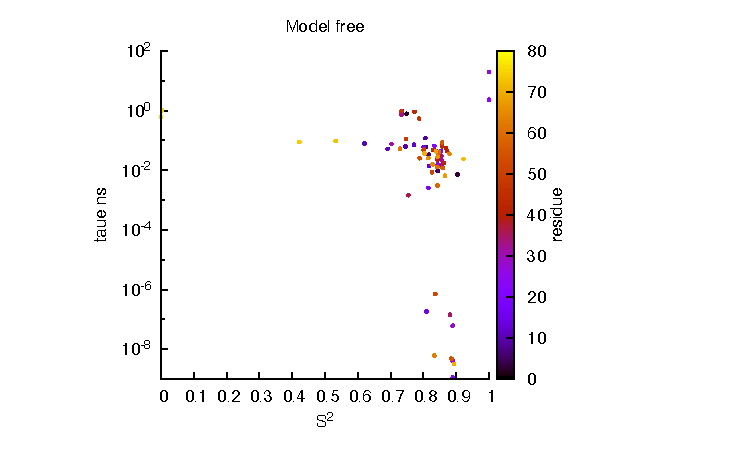
\includegraphics[width=0.495000\textwidth]{figGlobFreeAx3.pdf}
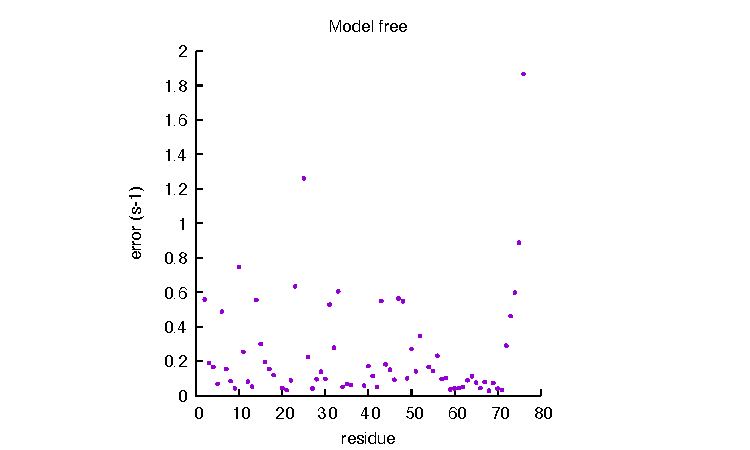
\includegraphics[width=0.495000\textwidth]{figGlobFreeAx4.pdf}
\end{figure} 
\noindent Parameters $P$: 142

$\tau_c$ global: 4.002 ns

shape global: 1.184

\noindent Datapoints $N$: 210

$\chi^2/N$: 27.894

$\chi^2/(N-P)$: 86.144

RMSD:   0.1510 s$^{-1}$

\end{document}
